\subsection{Simon's Algorithm}\label{sec:simons-algorithm}

\subsubsection{Problem Definition and Classical Solution}\label{sec:simons-algorithm-problem-definition-and-classical-solution}

Simon's algorithm is another \textbf{hidden-bitstring problem}, so there is a similar structure with Bernstein-Vazirani (\autopageref{sec:bernstein-vazirani-algorithm}). However, the way the hidden string is encoded is completely different. In Bernstein-Vazirani we had:
\begin{equation*}
    f_w (x) = w \cdot x \mod 2
\end{equation*}
And wanted to recover $w$ by querying the oracle. In Simon's problem, the hidden bitstring instead represents an \textbf{XOR period} of a function.

\highspace
\begin{flushleft}
    \textcolor{Red2}{\faIcon{exclamation-triangle} \textbf{The Problem}}
\end{flushleft}
We are given a black-box function:
\begin{equation*}
    f: \{0,1\}^{n} \to \{0,1\}^{n}
\end{equation*}
So both the input and output are $n$-bit strings. There exists an unknown, non-zero bitstring:
\begin{equation*}
    a \in \{0,1\}^{n}, \quad a \neq 0^n
\end{equation*}
That we \textbf{want to discover}. The function is promised to satisfy:
\begin{equation}\label{eq:simons-promise}
    f(x) = f(y) \iff x = y \quad \text{or} \quad x = y \oplus a
\end{equation}
Where $\oplus$ is the bitwise XOR operation:
\begin{center}
    \begin{tabular}{@{} c c c @{}}
        \toprule
        $y$ & $a$ & $y \oplus a$ \\
        \midrule
        0 & 0 & 0 \\
        0 & 1 & 1 \\
        1 & 0 & 1 \\
        1 & 1 & 0 \\
        \bottomrule
    \end{tabular}
\end{center}

\noindent
This is \textbf{Simon's promise}. The \textbf{goal} of Simon's algorithm is therefore simply to \textbf{find the hidden bitstring} $a$. But let's understand \textbf{\emph{what the promise actually means}} before thinking about how to solve the problem.

\highspace
\begin{flushleft}
    \textcolor{Green3}{\faIcon{question-circle} \textbf{What does Simon's promise mean?}}
\end{flushleft}
Suppose $n = 2$. Then there are four possible inputs: $00$, $01$, $10$, and $11$. We \textbf{don't know how $f$ was constructed}. We can only give it inputs and observe the outputs. For example, imagine this black box function:
\begin{center}
    \begin{tabular}{@{} c c @{}}
        \toprule
        $x$ & $f(x)$ \\
        \midrule
        00 & 10 \\
        01 & 10 \\
        10 & 01 \\
        11 & 01 \\
        \bottomrule
    \end{tabular}
\end{center}

\noindent
Notice that the outputs repeat:
\begin{equation*}
    f(00) = f(01) = 10 \quad \text{and} \quad f(10) = f(11) = 01
\end{equation*}
So there are two \textbf{collisions}: $00$ and $01$ collide, and $10$ and $11$ collide.

\highspace
\textcolor{Green3}{\faIcon{check} \textbf{Simon tells us that these collisions aren't random.}} The Simon's promise tells us that exists some secret nonzero string $a$ such that whenever two \textbf{different} inputs have the same output, they differ exactly by $a$. So look at out first collision: $f(00) = f(01)$. The two inputs are $00$ and $01$. If we XOR them together, we get:
\begin{equation*}
    00 \oplus 01 = 01
\end{equation*}
Therefore the secret string $a$ must be $01$. Now check the other collision: $f(10) = f(11)$. Again XOR the inputs:
\begin{equation*}
    10 \oplus 11 = 01
\end{equation*}
Same result! So we have found the hidden string $a = 01$.

\highspace
\textcolor{Green3}{\faIcon{book} \textbf{Another way to see it.}} If the hidden string is $a = 01$, then Simon promises that every $x$ has a ``partner'' $x \oplus a$ that collides with it. Start with $x = 00$:
\begin{equation*}
    00 \oplus 01 = 01
\end{equation*}
Therefore Simon's promise requires:
\begin{equation*}
    f(00) = f(01)
\end{equation*}
Let's continue with $x = 10$:
\begin{equation*}
    10 \oplus 01 = 11
\end{equation*}
So Simon's promise requires:
\begin{equation*}
    f(10) = f(11)
\end{equation*}
And that's exactly what we observed in the table above. So the promise is satisfied.

\highspace
\textcolor{Green3}{\faIcon{question-circle} \textbf{What if $a$ were different?}} Suppose instead that the hidden string was $a = 11$. Then the pairs would change. For $x = 00$:
\begin{equation*}
    00 \oplus 11 = 11
\end{equation*}
So Simon's promise would require:
\begin{equation*}
    f(00) = f(11)
\end{equation*}
And for $x = 01$:
\begin{equation*}
    01 \oplus 11 = 10
\end{equation*}
So Simon's promise would require:
\begin{equation*}
    f(01) = f(10)
\end{equation*}
But this is \textbf{not what we observed} in the table above. Therefore $a$ cannot be $11$. In fact, if we check all the other possibilities, we will find that $a = 01$ is the only one that satisfies Simon's promise.

\highspace
Finally, suppose \textbf{we don't know $a$}. We query the mysterious black-box function and observe the outputs:
\begin{equation*}
    f(01) = 10 \quad \text{and} \quad f(00) = 10
\end{equation*}
We have found a collision! Simon's promise guarantees that two different inputs with the same output must differ by the hidden string $a$. So we can XOR the inputs together to find $a$:
\begin{equation*}
    01 \oplus 00 = 01
\end{equation*}
And we solved the problem.

\highspace
\textcolor{Green3}{\faIcon{check-circle} \textbf{If we find a collision, we immediately find $a$.}} In the previous explanation, we found a collision by brute force. We queried the function for all possible inputs and observed the outputs. But this is \textbf{not efficient}! Suppose classically we query the function and happen to find two different inputs $x_1 \neq x_2$ that collide:
\begin{equation*}
    f(x_1) = f(x_2)
\end{equation*}
Simon's promise guarantees that:
\begin{equation*}
    x_2 = x_1 \oplus a
\end{equation*}
But then we can isolate $a$ to find a general formula for the hidden string:
\begin{align*}
    x_2 &= x_1 \oplus a \\
    x_2 \oplus x_1 &= x_1 \oplus a \oplus x_1 \\
    &\downarrow \quad x_1 \oplus x_1 = 0 \\
    x_2 \oplus x_1 &= a
\end{align*}
And we obtain the hidden string $a$:
\begin{equation}
    a = x_1 \oplus x_2
\end{equation}
And this is extremely important, because suppose we query the oracle and eventually discover a collision:
\begin{equation*}
    f(001) = f(110)
\end{equation*}
Then immediately we can find the hidden string:
\begin{equation*}
    a = 001 \oplus 110 = 111
\end{equation*}
So the classical problem can be rephrased as: \emph{\textbf{how many queries do ew need before we find two different inputs producing the same output?}}

\newpage

\begin{flushleft}
    \textcolor{Green3}{\faIcon{equals} \textbf{The equivalent formulation}}
\end{flushleft}
The promise can therefore be written more intuitively as:
\begin{equation}
    f(x) = f\left(x \oplus a\right), \quad \forall x \in \{0,1\}^{n}
\end{equation}
Take an arbitrary $x$. Its ``partner'' is $y = x \oplus a$. By Simon's promise:
\begin{equation*}
    f(x) = f(y), \quad \Rightarrow \quad f(x) = f\left(x \oplus a\right)
\end{equation*}
This is why $a$ is often called the \textbf{hidden XOR period} (i.e., because $f$ repeats itself every $a$). It plays a role analogous to an ordinary period. For example, for a familiar periodic function we might have: $f(x) = f(x + r)$ for some period $r$.

\highspace
\begin{flushleft}
    \textcolor{Green3}{\faIcon{question-circle} \textbf{Why is the function 2-to-1?}}
\end{flushleft}
A function is called \textbf{2-to-1} if \hl{every output has exactly two inputs that map to it.} For example:
\begin{equation*}
    f(00) = 10 \quad \text{and} \quad f(01) = 10
\end{equation*}
Here, \textbf{two inputs} $00$ and $01$ produce \textbf{one output} $10$. Now, \hl{Simon's promise guarantees that this happens systematically.} Suppose $a = 01$ and take $x = 00$. Its partner is:
\begin{equation*}
    x \oplus a = 00 \oplus 01 = 01
\end{equation*}
And Simon's promise says:
\begin{equation*}
    f(00) = f(01)
\end{equation*}
So that's one pair of inputs producing the same output: $\left\{00, 01\right\}$. Now take $x = 10$. Its partner is:
\begin{equation*}
    x \oplus a = 10 \oplus 01 = 11
\end{equation*}
And Simon's promise says:
\begin{equation*}
    f(10) = f(11)
\end{equation*}
So that's another pair of inputs producing the same output: $\left\{10, 11\right\}$. Therefore, for $n=2$, we might have the following mapping:
\begin{center}
    \begin{tabular}{@{} c c @{}}
        \toprule
        Inputs & Output \\
        \midrule
        00, 01 & 10 \\
        10, 11 & 01 \\
        \bottomrule
    \end{tabular}
\end{center}

\noindent
There are 4 inputs but only 2 distinct outputs. So the function is 2-to-1.

\highspace
In general, there are \hl{$2^n$ possible $n$-bit inputs.} Since we group them \textbf{two at a time}:
\begin{equation}\label{eq:distinct-outputs}
    \frac{2^{n}}{2} = 2^{n-1}
\end{equation}
There are \hl{$2^{n-1}$ distinct outputs.} For example, for $n=2$ we have $2^2 = 4$ inputs, which are grouped into $2^{2-1} = 2$ pairs.

\newpage

\begin{flushleft}
    \textcolor{Red2}{\faIcon{hourglass-half} \textbf{Deterministic classical solution}}
\end{flushleft}
We don't know $a$, but we know that if we ever find a collision:
\begin{equation*}
    f(x_1) = f(x_2), \quad x_1 \neq x_2
\end{equation*}
Then we're finished:
\begin{equation*}
    a = x_1 \oplus x_2
\end{equation*}
So, \textbf{\emph{how many oracle queries do we need to find a collision?}}

\highspace
Suppose $n=3$. There are $2^3 = 8$ possible inputs. Because Simon's function is 2-to-1, those 8 inputs are grouped into $2^{3-1} = 4$ pairs of hidden pairs. For example, perhaps $a = 001$. Then the pairs are:
\begin{equation*}
    \left\{000, 001\right\}, \quad \left\{010, 011\right\}, \quad \left\{100, 101\right\}, \quad \left\{110, 111\right\}
\end{equation*}
Each pair produces one common output. Now imagine we're extremely unlucky (\textbf{worst-case scenario}). We query the oracle and get $000$, then $010$, then $100$, and then $110$. We've made \textbf{4 queries}, but notice what happened: we selected exactly \textbf{one member from each pair}. Therefore we haven't seen a collision yet. But now we've exhausted all 4 pairs. \emph{What happens with query number 5?} Whatever remaining input we choose, it must belong to one of the pairs we've already touched.

\highspace
For example, if we choose $101$, we already queried its partner $100$:
\begin{equation*}
    f(100) = f(101)
\end{equation*}
Collision! Therefore for $n=3$, we need at most $2^{3-1} + 1 = 5$ queries to find a collision.

\highspace
In general, with $n$ bits there are $2^{n}$ inputs. Because they come in pairs, there are $2^{n-1}$ pairs. In the \textbf{worst possible case}, we first query one member of each pair $2^{n-1}$ times, and we still haven't found a collision. But the next query must be a member of one of the pairs we've already seen, so we will find a collision. Therefore, in the worst case, we need at most:
\begin{equation}
    2^{n-1} + 1 = O(2^n)
\end{equation}
\begin{remarkbox}[: Why do we write $O(2^n)$?]
    Because Big-O ignores constant factors and lower-order constants. We have:
    \begin{equation*}
        2^{n-1} + 1
    \end{equation*}
    But we can rewrite $2^{n-1}$ as:
    \begin{equation*}
        2^{n-1} = \frac{2^n}{2}
    \end{equation*}
    Therefore, we can write:
    \begin{equation*}
        2^{n-1} + 1 = \frac{1}{2} \cdot 2^n + 1
    \end{equation*}
    And in Big-O notation, we ignore constant factors and lower-order terms, so we write:
    \begin{equation*}
        2^{n-1} + 1 = O\left(2^n\right)
    \end{equation*}
    For example:
    \begin{center}
        \begin{tabular}{@{} c c @{}}
            \toprule
            $n$ & $2^{n-1} + 1$ \\
            \midrule
            3 & 5 \\
            10 & 513 \\
            20 & 524'289 \\
            30 & 536'870'913 \\
            \bottomrule
        \end{tabular}
    \end{center}
    It grows exponentially with $n$.
\end{remarkbox}

\begin{flushleft}
    \textcolor{Red2}{\faIcon{dice} \textbf{Randomized classical solution}}
\end{flushleft}
The deterministic classical solution is \textbf{exponential}, but we can do better with a \textbf{randomized approach}. The deterministic result asks: \emph{how many queries do we need to guarantee a collision even if we're maximally unlucky?} The answer is $2^{n-1} + 1$, $O(2^n)$. But now suppose we're willing to say: \emph{\textbf{we're choose inputs randomly. How many queries before a collision becomes likely?}} This is a classic \textbf{birthday problem}.

\highspace
The \definition{Birthday Problem} is a famous problem in probability theory. There are 365 possible birthdays. We might initially think ``\emph{to have a good chance that two people share a birthday, perhaps we need around 365 people}''. But that's not true. With only \textbf{23 people}, the probability that at least two share a birthday is already above 50\%.

\highspace
\emph{Why?} Because we're not comparing everyone against one particular person. We're comparing \textbf{every person with every other person}. With $k$ people, the number of pairs of people is:
\begin{equation*}
    \binom{k}{2} = \frac{k(k-1)}{2} \approx \frac{k^2}{2}
\end{equation*}
So the number of possible comparisons grows roughly like $k^2$. Therefore, the probability of a collision grows much faster than we might initially expect.

\highspace
\textcolor{Red2}{\faIcon{question-circle} \textbf{What plays the role of the 365 birthdays in Simon?}} In Simon, the ``birthday categories'' (i.e., the number of distinct outputs) are the $2^{n-1}$ \textbf{input pairs} created by the hidden string $a$. Suppose we have $2^{n}$ possible inputs. Simon's promise partitions them into $2^{n-1}$ pairs:
\begin{equation*}
    \left\{
        x, x \oplus a
    \right\}
\end{equation*}
Both members of a pair give the same output:
\begin{equation*}
    f(x) = f(x \oplus a)
\end{equation*}
So finding a collision is equivalent to randomly selecting \textbf{both members of one of these hidden pairs}. Now suppose we randomly query $k$ distinct inputs. Among those $k$ inputs there are:
\begin{equation*}
    \binom{k}{2} = \frac{k(k-1)}{2} \approx \frac{k^2}{2}
\end{equation*}
Possible pairs of queried inputs. For any particular pair of random distinct inputs $x_i,x_j$, the chance that they happen to be Simon partners is roughly $\frac{1}{2^{n}}$. Because once $x_i$ is chosen, there is exactly \textbf{one special other input} $x_i \oplus a$ among roughly $2^{n}$ possible inputs. Therefore, with approximately $\frac{k^2}{2}$ opportunities for a collision, the expected number of collisions is roughly:
\begin{equation*}
    \frac{k^2}{2} \cdot \frac{1}{2^{n}}
\end{equation*}
A collision becomes reasonably likely when this reaches order 1:
\begin{equation*}
    \frac{k^2}{2^{n+1}} \sim 1
\end{equation*}
Ignoring constant factors for complexity:
\begin{equation*}
    k^2 \sim 2^{n}
\end{equation*}
Therefore:
\begin{equation}
    k \sim \sqrt{2^{n}} = 2^{n/2} \quad \Rightarrow \quad k = O(2^{n/2})
\end{equation}
In contrast to the deterministic classical solution, which requires $O(2^n)$ queries, the randomized classical solution ``\emph{only}'' requires $O(2^{n/2})$ queries. This is a \textbf{quadratic speedup} over the deterministic approach.

\highspace
\begin{examplebox}[: $n=10$]
    Suppose $n=10$. Then there are $2^{10} = 1024$ possible inputs. Because Simon's function is 2-to-1, those 1024 inputs are grouped into $2^{10-1} = 512$ hidden pairs. If we randomly query about:
    \begin{equation*}
        k = \sqrt{2^{10}} = \sqrt{1024} = 32
    \end{equation*}
    Inputs, those 32 inputs create roughly:
    \begin{equation*}
        \binom{32}{2} = \frac{32 \cdot 31}{2} = 496
    \end{equation*}
    Different pairs of queried inputs. So despite querying only about 32 of the 1024 inputs, we already have \textbf{hundreds of chances} that one of our queried pairs happens to be a hidden Simon pair. That's the birthday-paradox effect. Therefore, with only about 32 random queries, we have a good chance of finding a collision and discovering the hidden string $a$.
\end{examplebox}

\newpage

\begin{flushleft}
    \textcolor{Green3}{\faIcon{check-circle} \textbf{What Simon's quantum algorithm changes}}
\end{flushleft}
Simon found a way to \textbf{avoid searching directly for a collision}. The quantum algorithm uses \hl{only $O(n)$ oracle queries.} But there is an important difference from Bernstein-Vazirani. In \textbf{Bernstein-Vazirani}, we \textbf{queried} the oracle \textbf{once} and got the hidden string $w$ immediately. Instead, in Simon's algorithm, \textbf{each execution gives us some bitstring} $y$ satisfying:
\begin{equation*}
    a \cdot y = 0 \mod 2
\end{equation*}
That's one equation involving the unknown hidden string $a$. We need to repeat the algorithm $O(n)$ times until we have enough independent equations to solve for $a$. We'll derive \emph{why the circuit produces exactly these equations} later, but for now let's just accept that this is what happens. The important point is that Simon provides an \textbf{exponential query-complexity advantage} over classical algorithms.

\begin{figure}[htp]
    \centering
    \tikzsetnextfilename{simons-query-complexity}
    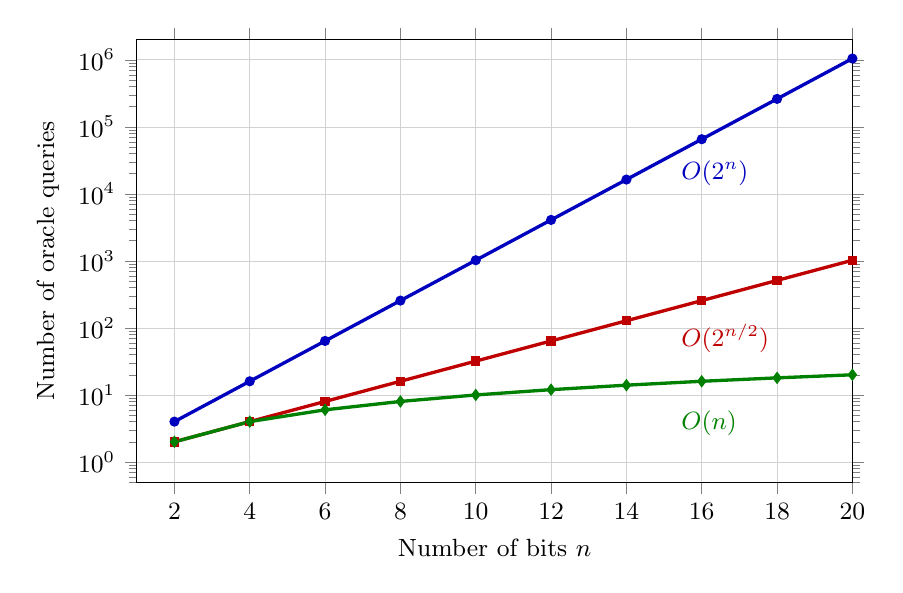
\begin{tikzpicture}
        \begin{semilogyaxis}[
                width=0.88\textwidth,
                height=7.2cm,
                xlabel={Number of bits $n$},
                ylabel={Number of oracle queries},
                xmin=1,
                xmax=20,
                ymin=0.5,
                ymax=2e6,
                xtick={2,4,6,8,10,12,14,16,18,20},
                % Major grid only
                xmajorgrids=true,
                ymajorgrids=true,
                xminorgrids=false,
                yminorgrids=false,
                major grid style={
                    line width=0.3pt,
                    draw=gray!35
                },
                axis line style={black},
                tick align=outside,
                label style={font=\small},
                tick label style={font=\small},
                clip=false,
            ]

            % ---------------------------------------------------------
            % Deterministic classical: O(2^n)
            % ---------------------------------------------------------
            \addplot[
                blue!75!black,
                very thick,
                mark=*,
                mark size=1.2pt,
                domain=2:20,
                samples=10
            ] {2^x};

            \node[
                anchor=west,
                text=blue!75!black,
                font=\small
            ] at (axis cs:15.2,2.0e4)
            {$O(2^n)$};

            % ---------------------------------------------------------
            % Randomized classical: O(2^{n/2})
            % ---------------------------------------------------------
            \addplot[
                red!75!black,
                very thick,
                mark=square*,
                mark size=1.1pt,
                domain=2:20,
                samples=10
            ] {2^(x/2)};

            \node[
                anchor=west,
                text=red!75!black,
                font=\small
            ] at (axis cs:15.2,70)
            {$O(2^{n/2})$};

            % ---------------------------------------------------------
            % Simon's quantum algorithm: O(n)
            % ---------------------------------------------------------
            \addplot[
                green!50!black,
                very thick,
                mark=diamond*,
                mark size=1.3pt,
                domain=2:20,
                samples=10
            ] {x};

            % Label deliberately placed BELOW the green curve
            \node[
                anchor=north west,
                text=green!50!black,
                font=\small
            ] at (axis cs:15.2,8)
            {$O(n)$};

        \end{semilogyaxis}
    \end{tikzpicture}

    \caption{
        \textbf{Query-complexity scaling for Simon's problem.}
        A deterministic classical strategy requires exponentially many
        oracle queries, while randomized classical search reduces the
        complexity to approximately $O(2^{n/2})$ through the
        birthday-paradox effect. Simon's quantum algorithm requires only
        $O(n)$ oracle queries.
    }
    \label{fig:simon-query-complexity}
\end{figure}

\newpage

\begin{table}[!htp]
    \centering
    \begin{tabular}{@{} l l l @{}}
        \toprule
        & Bernstein-Vazirani & Simon \\
        \midrule
        Hidden string & $w$ & $a \neq 0$ \\[.3em]
        Structure & $f_w(x) = w \cdot x$ & $f(x) = f(x \oplus a)$ \\[.3em]
        Meaning & hidden coefficients & hidden XOR period \\[.3em]
        Classical & $O(n)$ queries & randomized $O(2^{n/2})$ \\[.3em]
        Quantum & $O(1)$ queries & $O(n)$ queries \\[.3em]
        One run gives & $w$ & $y$ s.t. $a \cdot y = 0$ \\[.3em]
        Post-processing & none & solve $O(n)$ equations for $a$ \\
        \bottomrule
    \end{tabular}
    \caption{
        \textbf{Comparison of Bernstein-Vazirani and Simon's.}
        It's interesting to note that \textbf{Simon uses more quantum queries than Bernstein-Vazirani},
        but achieves a much stronger asymptotic separation (exponential vs. linear)
        between classical and quantum query complexity.
    }
    \label{tab:simon-bernstein-vazirani}
\end{table}

\begin{takeawaysbox}
    Simon's algorithm considers a function $f:\{0,1\}^n\rightarrow\{0,1\}^n$ for which there exists an unknown non-zero bitstring $a$ satisfying $f(x)=f(y)$ if and only if $x=y$ or $x=y\oplus a$. Therefore, $f(x)=f(x\oplus a)$, and $a$ represents a hidden XOR period. The goal is to recover $a$. Classically, finding a collision requires $O(2^{n/2})$ randomized queries, whereas Simon's quantum algorithm requires $O(n)$ oracle queries.

    \highspace
    Also, the classical algorithm \textbf{searches for such a collision}:
    \begin{equation*}
        f(x_1) = f(x_2), \quad x_1 \neq x_2 \quad \Rightarrow \quad a = x_1 \oplus x_2
    \end{equation*}
    Simon's quantum algorithm, instead, will take a completely different route: it will extract \textbf{linear constrains on $a$} using interference.
\end{takeawaysbox}